%%%% Paramétrage du TD %%%%
\def\xxactivite{ \ifprof {Application 4 -- Corrigé } \else  \ifcolle Colle \else Application 4\fi \fi} % \normalsize \vspace{-.4cm}
\def\xxauteur{\textsl{Xavier Pessoles}}

\def\xxnumchapitre{Chapitre 1 \& 2 \vspace{.2cm}}
\def\xxchapitre{\hspace{.12cm} Chaînes de solides}



\def\xxcompetences{%
\footnotesize{
\textsl{%
\textbf{Savoirs et compétences :}\\
\vspace{-.2cm}
\begin{itemize}[label=\ding{112},font=\color{ocre}] 
\item \textit{Mod2.C34} : chaînes de solides;
\item \textit{Mod2.C34} : degré de mobilité du modèle;
\item \textit{Mod2.C34} : degré d’hyperstatisme du modèle;
%\item \textit{Mod2.C34.SF1} : déterminer les conditions géométriques associées à l’hyperstatisme;
%\item \textit{Mod2.C34} : résoudre le système associé à la fermeture cinématique et en déduire le degré de mobilité et d’hyperstatisme.
\end{itemize}}}}

\def\xxtitreexo{Appareil de mammographie « ISIS » (General Electric)}
\def\xxsourceexo{\hspace{.2cm} \footnotesize{Centrale MP 2004}}

\def\xxfigures{
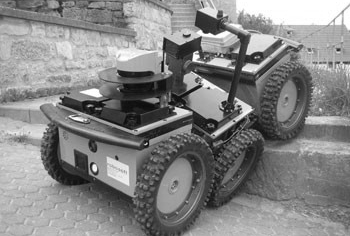
\includegraphics[width=.5\textwidth]{fig_00}
}%figues de la page de garde

\input{\repRel/Style/pagegarde_TD}
\setcounter{numques}{0}

\setlength{\columnseprule}{.1pt}

\pagestyle{fancy}
\thispagestyle{plain}


\vspace{5.2cm}

\def\columnseprulecolor{\color{ocre}}
\setlength{\columnseprule}{0.4pt} 

%%%%%%%%%%%%%%%%%%%%%%%

\setcounter{exo}{0}

\ifprof
\else
\begin{multicols}{2}
\fi


\section*{Mise en situation}

\ifprof
\else

\ifcolle
\else
Le mammographe est utilisée pour rechercher la présence d’une tumeur dans un sein. Il est constitué des éléments génériques suivants.

\begin{center}
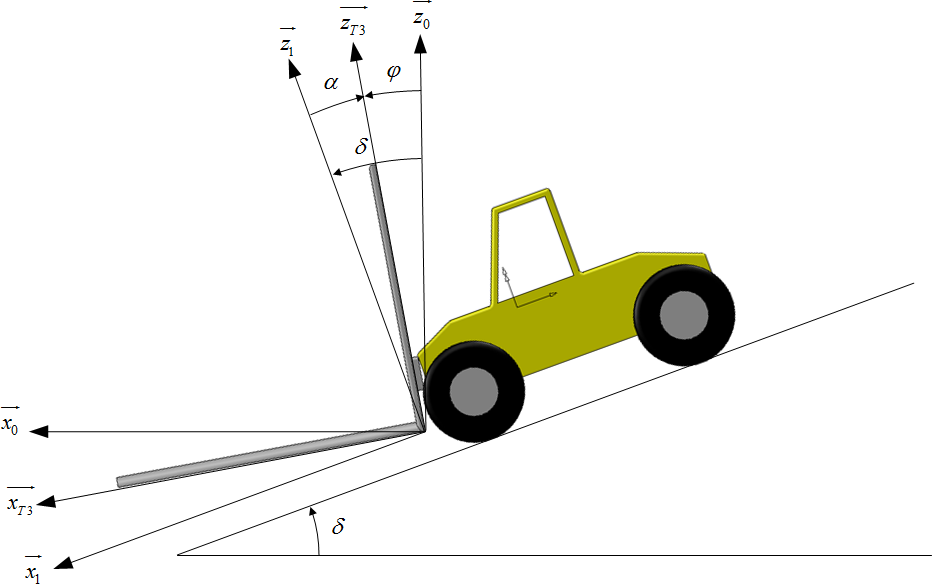
\includegraphics[width=\linewidth]{fig_02}
%\textit{}
\end{center}


Un ascenseur en liaison glissière de direction verticale par rapport à la partie fixe du mammographe (bâti). Cette mobilité permet d’adapter le mammographe à la taille de la patiente. L’ascenseur supporte les éléments suivants : la « tête RX » qui permet d’émettre les rayons X et un collimateur qui permet de contrôler le faisceau afin d’optimiser le cliché. Le réglage angulaire de la tête RX est réalisé par un pivotement autour de l’axe de rotation du mammographe.
La tête RX est donc en liaison pivot par rapport à l’ascenseur.


Le « bucky » sert de surface d’appui au sein et de support au film ou au capteur
d’images. %Il peut également recevoir le stéréotix permettant de réaliser une biopsie (prélèvement au niveau de la tumeur). 
Le réglage angulaire du
bucky est réalisé par un pivotement autour de l’axe de rotation du mammographe.
Le bucky est en liaison pivot par rapport à l’ascenseur.

La « plaque de pression » permet de comprimer le sein et de le maintenir en
position afin d’avoir une meilleure qualité de l’image. Elle fait l’objet d’une
liaison glissière par rapport au bucky.
À noter que les réglages angulaires des deux liaisons
pivots sont indépendants. On peut, par exemple, faire
tourner la tête sans faire tourner le bucky.
%
%Deux types d’examens radiologiques existent :
%\begin{itemize}
%\item le « screening » consiste en la prise de plusieurs clichés du sein suivant différents points de vue indépendants.
%Cet examen est 
%%C’est le premier examen radiologique effectué sur un sein. En particulier, c’est la procédure 
%utilisé lors des campagnes de dépistage systématique. En cas de diagnostic positif, l’examen de stéréatoxie peut être envisagé;
%\item la « stéréotaxie » consiste également en la prise de plusieurs clichés mais sans modifier le positionnement
%du sein sur le mammographe ni sa mise en pression. Les différentes vues 2D ainsi obtenues
%permettent d’identifier en 3D le positionnement précis de la tumeur. Les coordonnées de la tumeur sont
%alors communiquées au « stéréotix » afin de réaliser la biopsie avec précision.
%\end{itemize}

%%La chaîne image permet l’acquisition d’images numériques. Cette évolution technologique permet l’utilisation d’un logiciel capable de traiter l’image afin d’aider le radiologue dans la recherche des tumeurs de petites dimensions.

%
%\begin{center}
%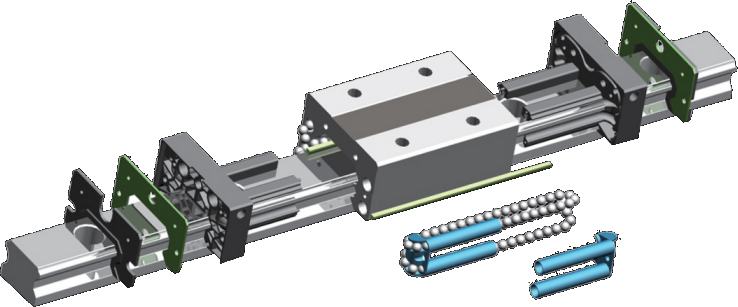
\includegraphics[width=.3\linewidth]{fig_03}
%\hspace{1cm}
%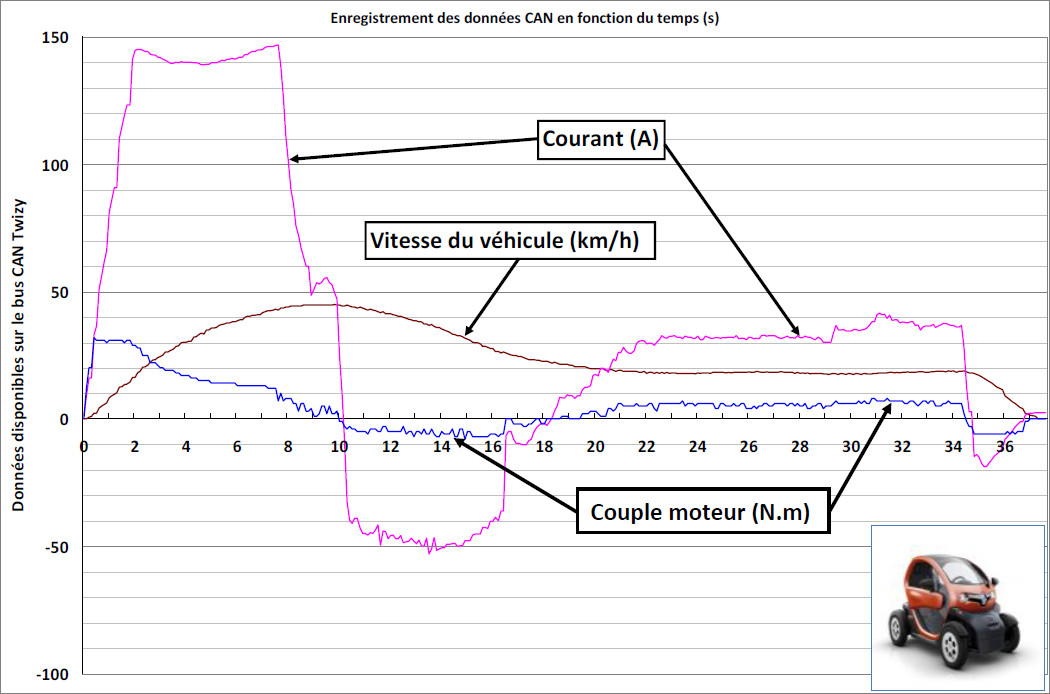
\includegraphics[width=.3\linewidth]{fig_04}
%%\textit{}
%\end{center}
\fi

\fi

%\section*{Étude de l’architecture du mammographe ISIS}
%
%\begin{obj}
%L’objectif de cette étude est l’identification de la structure cinématique du mammographe.
%\end{obj}
%
%On peut hiérarchiser les fonctions décrivant un examen de type «~screening~».
%\begin{center}
%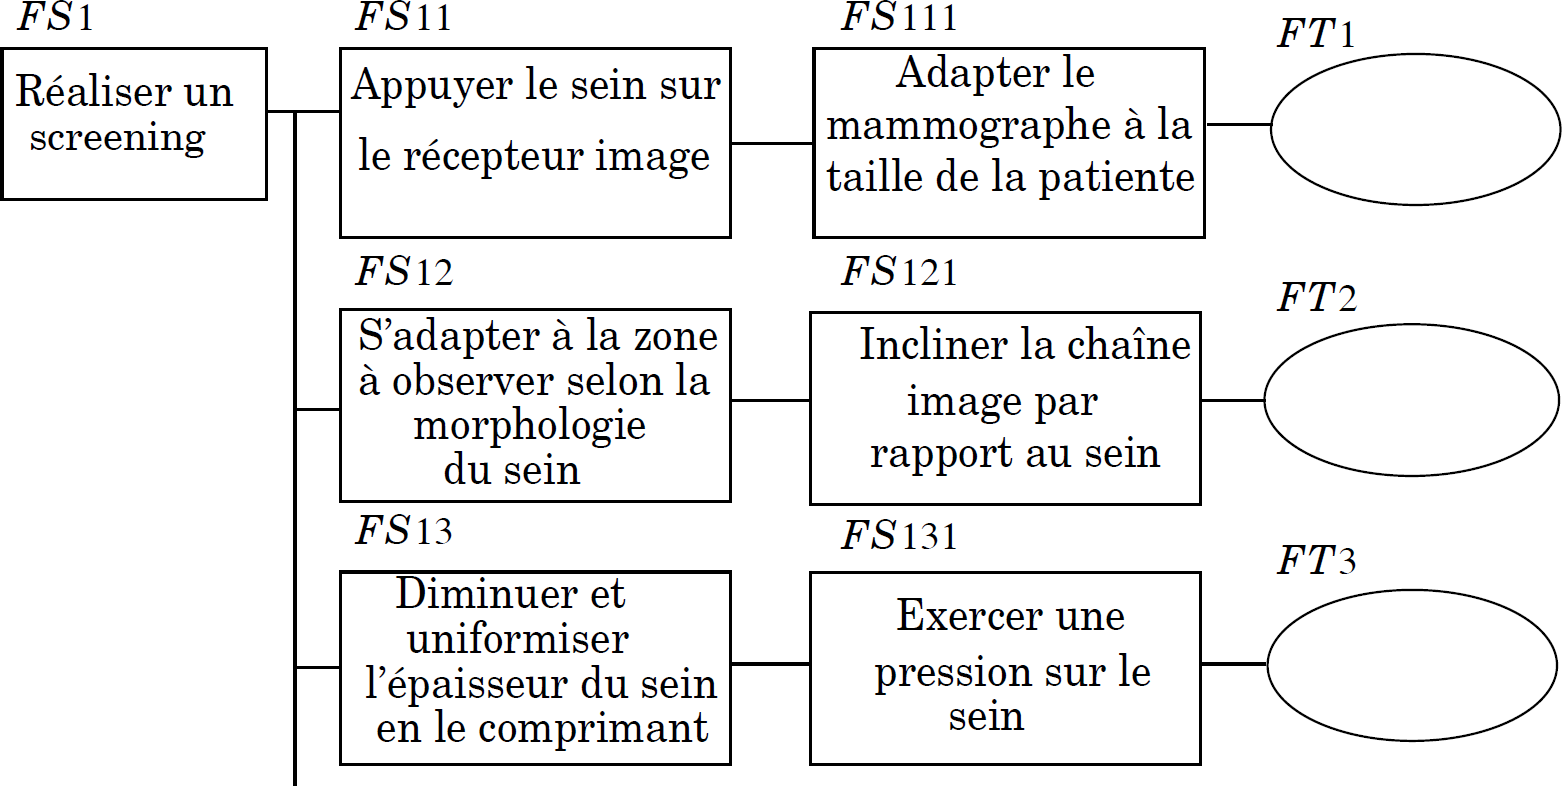
\includegraphics[width=\linewidth]{fig_05_bis}
%%\textit{}
%\end{center}
%
%\question{Dans le cas d’un examen de type «~screening~», préciser le mouvement associé à la réalisation de chaque fonction technique FT1, FT2 et FT3. Pour chaque mouvement, indiquer si c’est une translation ou une rotation, la direction ou l’axe du mouvement, le (ou les solides) en mouvement relatif ainsi que le solide par rapport auquel il a lieu.}
%\ifprof
%\begin{corrige}~\\
%\end{corrige}
%\else
%\fi
%
%
%
%\question{Par quel mouvement faut-il compléter la cinématique précédente pour
%que le mammographe permette également la réalisation d’un examen de type « stéréotaxie » ? Indiquer si c’est une
%translation ou une rotation, la direction ou l’axe du mouvement, le (ou les solides) en mouvement relatif ainsi que le
%solide par rapport auquel il a lieu.}
%\ifprof
%\begin{corrige}~\\
%\end{corrige}
%\else
%\fi
%
%
%
%
%\question{Tracer le schéma cinématique en
%perspective du mammographe « ISIS »
%qui permet de réaliser les deux types
%d’examens.}
%\ifprof
%\begin{corrige}~\\
%\end{corrige}
%\else
%\fi
%
%\begin{center}
%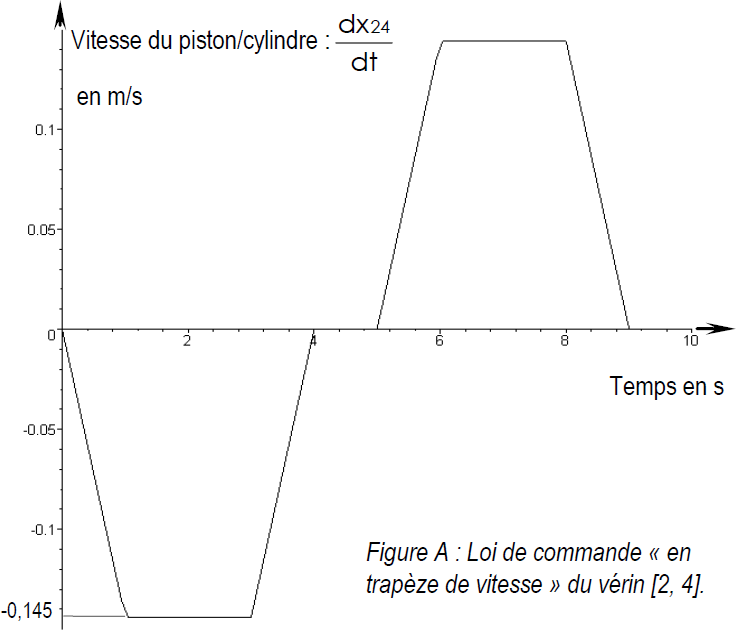
\includegraphics[width=.5\linewidth]{fig_06}
%%\textit{}
%\end{center}

\subsection*{Analyse de la fonction de service : « Adapter le
mammographe à la taille de la patiente » et de la fonction
technique associée : « faire monter et descendre
l’ascenseur »}
\ifprof
\else
Le mammographe doit être adapté à la taille de la patiente en faisant monter
ou descendre l’ascenseur. La liaison glissière de l’ascenseur par rapport à la partie
fixe du mammographe est réalisée par un guidage sur deux barres parallèles
fixées sur le bâti. Le déplacement de l’ascenseur est obtenu à partir d’un moteur
électrique qui entraîne en rotation une vis. La rotation de la vis entraîne ensuite
l’écrou sur lequel est fixé l’ascenseur.
Un vérin à gaz permet d’assister le moteur lors de la montée de l’ascenseur par
l’intermédiaire d’une poulie montée à l’extrémité de la tige du vérin à gaz et
d’une courroie crantée. Une des extrémités de la courroie est fixée sur le bâti du
mammographe et l’autre extrémité est liée à l’ascenseur.

\begin{center}
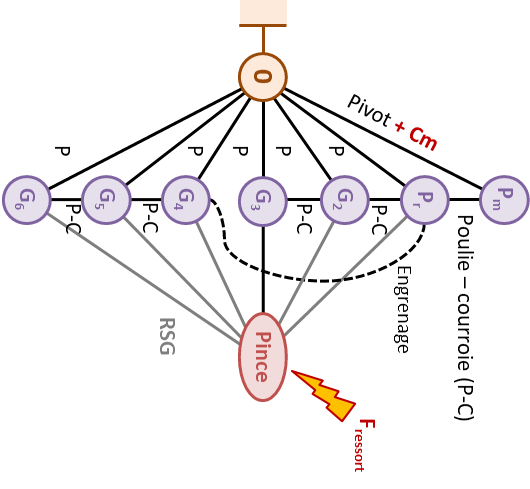
\includegraphics[width=.6\linewidth]{fig_07}
%\textit{}
\end{center}

\begin{center}
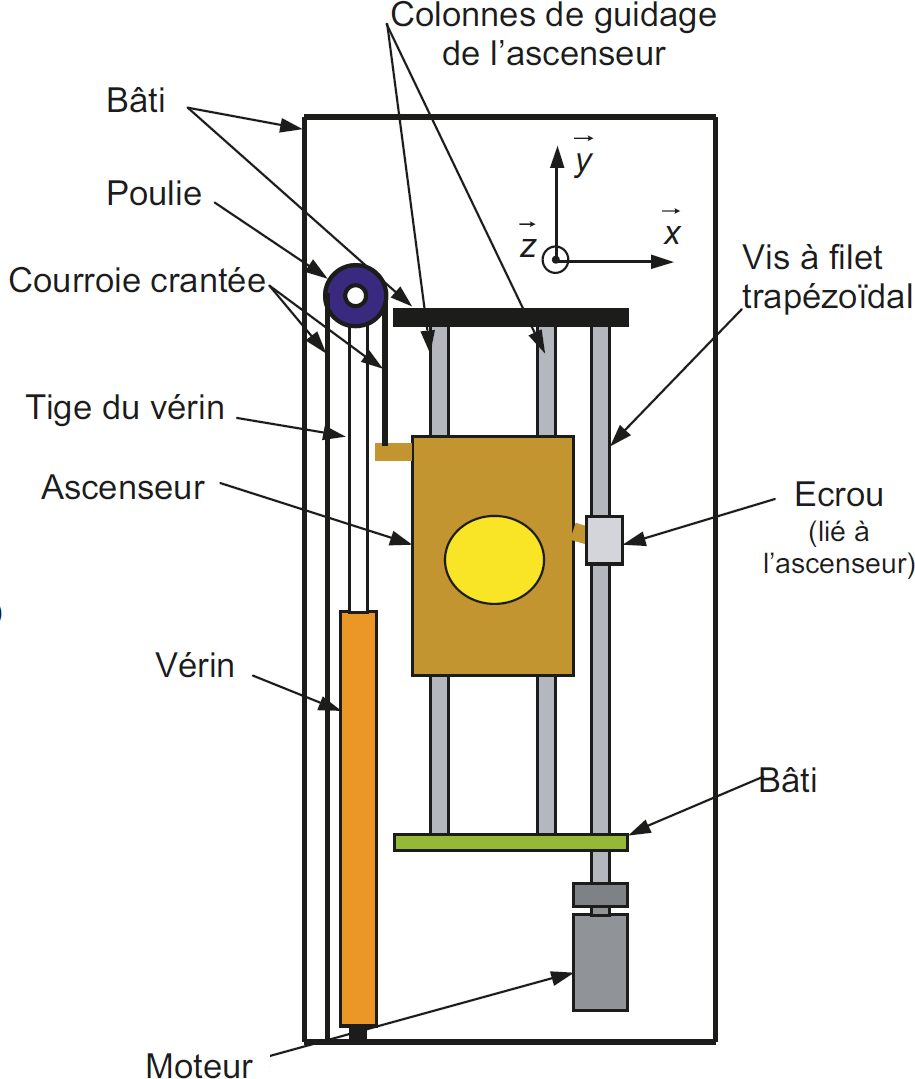
\includegraphics[width=.6\linewidth]{fig_08}
%\textit{}
\end{center}

\begin{center}
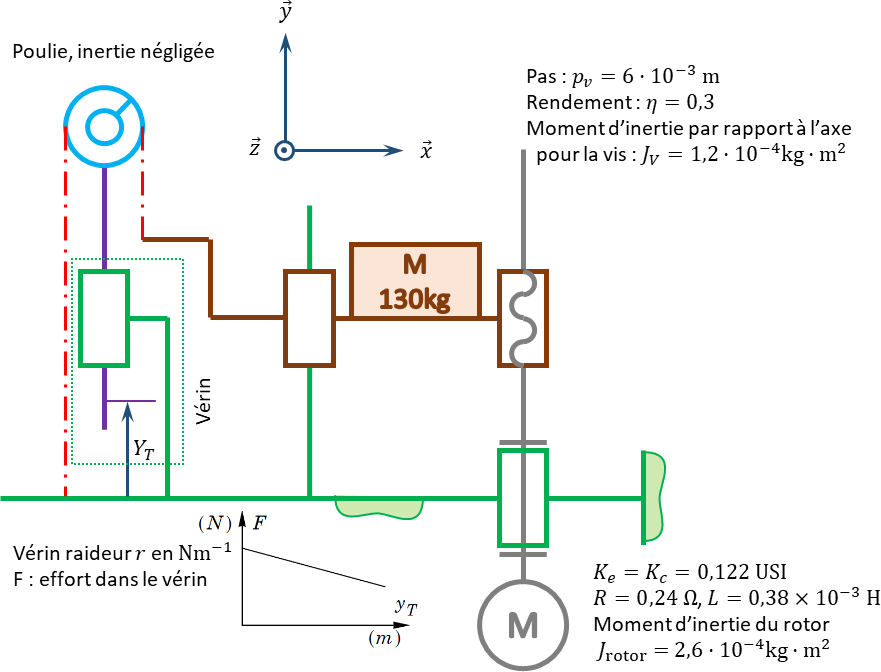
\includegraphics[width=\linewidth]{fig_10}
%\textit{}
\end{center}

\fi

%
%La figure précédente décrit la chaîne associée à la réalisation des fonctions techniques
%FT1 et FT2. Seuls les éléments intervenant dans FT1 sont repérés sur cette
%figure. Le schéma de principe de la chaîne associée à la
%réalisation de la fonction technique FT1 « Faire monter ou descendre
%l’ascenseur ».

\subsection*{Détermination de la motorisation}
\begin{obj}
L’objectif de cette étude est de valider la solution utilisant un vérin à gaz
pour assister le moteur, en la comparant à d’autres solutions
classiques : pas d’assistance, assistance à l’aide d’un contre-poids,
assistance à l’aide d’un ressort. Pour cela nous allons comparer les performances
minimales que doit avoir le moteur d’entraînement et vérifier
pour chaque cas la conformité au cahier des charges.
\end{obj}

\ifprof
\else
\begin{center}
\begin{tabular}{|p{.6\linewidth}|p{.3\linewidth}|}
\hline
\multicolumn{2}{|c|}{Faire monter ou descendre l'ascenseur} \\
\hline
Critères & Niveaux \\
\hline
Ne pas stresser la patiente en déplaçant trop rapidement l’ascenseur : limiter la vitesse de
déplacement rapide & $V_R=\SI{0,15}{m.s^{-1}}$ \\ \hline
Ne pas blesser la patiente lors de l’approche du bucky : respecter une vitesse lente $V_L$ lors de
l’accostage & $V_L=\SI{0,02}{m.s^{-1}}$ \\ \hline 
Respecter une course de réglage de la position de l’ascenseur & $\text{course} = \SI{0,8}{m}$  $\delta_{\text{course}}=\pm\SI{e-3}{m}$ \\ \hline
Atteindre rapidement la vitesse de déplacement rapide $V_R$: respecter
la durée $t_a$ de la phase d’accélération constante & $t_a=\SI{0,4}{s}$ (mini) \\
 \\ \hline
\end{tabular}
\end{center}


\fi

\question{Déterminer la fréquence de rotation du moteur $\omega$ en fonction de la vitesse de
déplacement $V$ de l’ascenseur. %Compléter alors, le bloc du schéma bloc dudocument réponse. 
En déduire la vitesse de rotation maximum $\omega_{\text{maxi}}$ que doit avoir le moteur, faire l’application numérique.}
\ifprof
\begin{corrige}~\\
On a $V=\omega \dfrac{p_v}{2\pi}$ et donc $\omega_{\text{maxi}} = V_R\dfrac{2\pi}{p_v}$.

Application numérique : $\omega_{\text{maxi}} = 0,15\dfrac{2\pi}{6\cdot 10^{-3}}=\SI{157}{rad.s^{-1}}$ $=\SI{1500}{tr.min^{-1}}$.
\end{corrige}
\else
\fi

\ifprof
\else
Pour déterminer les performances minimales du moteur, on étudie la phase de montée de l’ascenseur définie par :
\begin{enumerate}
\item départ en position basse ( $y=0$ à l’instant $t=0$);
\item mise en mouvement ascendant de l’ascenseur à accélération constante $a$ pour atteindre la vitesse $V_R$ rapide en respectant les contraintes du cahier des charges;
\item arrêt de l’ascenseur à la position $y=\SI{0,8}{m}$ (la phase de décélération est telle que la décélération est constante et sa durée égale à $t_a$).
\end{enumerate}
\fi

\question{Afin d’avoir une meilleure représentation de cette phase de montée de
l’ascenseur, représenter la loi d’accélération en fonction du temps ainsi que la loi
de vitesse et celle du déplacement $y$ de l’ascenseur. Indiquer les valeurs
numériques de l’accélération, de la durée de la phase d’accélération, du déplacement
réalisé pendant chaque phase de déplacement à accélération constante et de la durée du déplacement à vitesse constante.}
\ifprof
\begin{corrige}~\\

\begin{center}
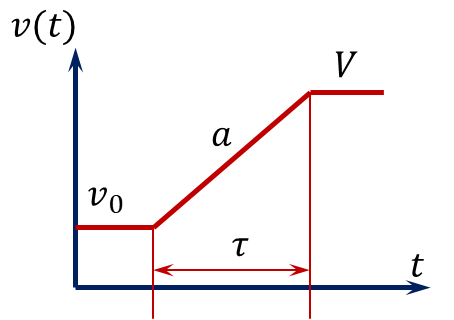
\includegraphics[width=.35\linewidth]{cor_01}
\end{center}

L’accélération $a_{\text{max}}$ est donnée par $a_{\text{max}} = \dfrac{V_R}{t_a}$ $=\dfrac{0,15}{0,4}$ $=\SI{0,375}{m.s^{-2}}$. 

Les distances parcourues correspondent à l'aire sous la courbe du profil de vitesse. La distance d'accélération et de décélération sont données par $d_a=\dfrac{1}{2}V_R t_a$ $=\dfrac{1}{2}0,15\times 0,4$ $=\SI{0,03}{m}$.

En conséquence, la distance à parcourir à vitesse constante est $d_c=0,8-2\times 0,03$ $=\SI{0,74}{m}$. Le temps pour parcourir cette distance est $t_c=\dfrac{d_c}{V_R}$ $=\dfrac{0,74}{0,15}$ $=\SI{4,13}{s}$.
\end{corrige}
\else
\fi

\subsection*{Solution sans assistance}
\ifprof
\else
On souhaite déterminer le couple moteur. Pour cela on propose d’appliquer le théorème de
l’énergie-puissance au système isolé $\Sigma$ (rotor du moteur + vis + ascenseur) en mouvement
par rapport au bâti supposé galiléen. 

\begin{center}
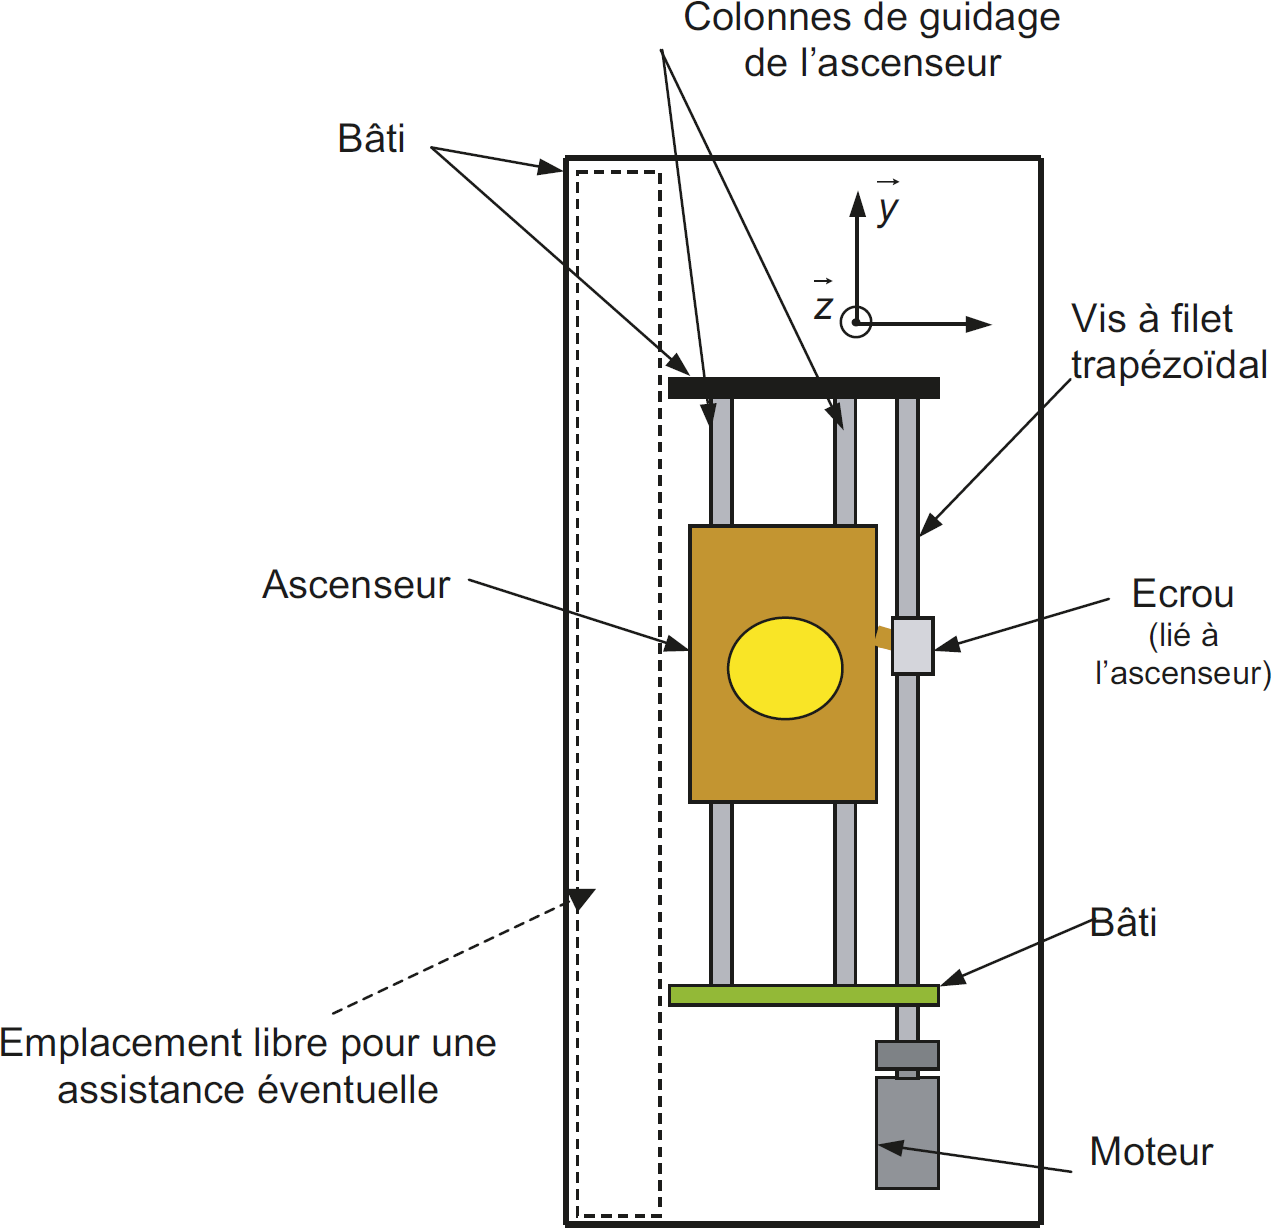
\includegraphics[width=\linewidth]{fig_10_bis}
%\textit{}
\end{center}

On notera :
\begin{itemize}
\item $\vect{g}=-g\vect{y}$ l’accélération de la pesanteur. On prendra $g=\SI{9,81}{m.s^{-2}}$;
\item $C$ le couple exercé par le stator sur le rotor du moteur.
\end{itemize}
\fi

\question{Déterminer l’énergie cinétique galiléenne, notée $\ec{\Sigma}{0}$, du système isolé. Mettre $\ec{\Sigma}{0}$ sous la forme : $\ec{\Sigma}{0} = \dfrac{1}{2}M_eV^2$. Donner l’expression littérale de la masse équivalente $M_e$ et faire l’application numérique.}
\ifprof
\begin{corrige}~\\
Calcul de l'énergie cinétique : $\ec{\Sigma}{0} = \dfrac{1}{2}\left( J_R+J_V\right) \left(  V\dfrac{2\pi}{p_v}\right)^2+\dfrac{1}{2}MV^2$ $= \dfrac{1}{2}\left(\left( J_R+J_V\right) \dfrac{4\pi^2}{p_v^2} +M \right)V^2$.

On a donc $M_e = \left( J_R+J_V\right) \dfrac{4\pi^2}{p_v^2} +M$ $=\left( 2,6\times 10^{-4}+1,2\times 10^{-4}\right) \dfrac{4\pi^2}{\left( 6\times 10^{-3}\right)^2} +130$
$=\left( 2,6\times 10^{-4}+1,2\times 10^{-4}\right) \dfrac{4\pi^2}{\left( 6\times 10^{-3}\right)^2} +150 = \SI{547}{kg}$.
\end{corrige}
\else
\fi


\question{En supposant que toutes les liaisons sont parfaites, appliquer le théorème de
l’énergie puissance au système isolé (rotor du moteur + vis + ascenseur). La
démarche suivie doit être clairement indiquée. En déduire l’expression littérale
de $C$ en fonction de $V$ et/ou de ses dérivées, $\omega$ et/ou ses dérivées n’apparaîtront
pas dans l’expression littérale de $C$.}
\ifprof
\begin{corrige}~\\
\begin{itemize}
\item On isole $\Sigma$. 
\item Bilan des puissances intérieures : liaisons parfaites $\mathcal{P}_{\text{int}} = 0$.
\item Bilan des puissances extérieures : 
\begin{itemize}
\item $\pext{\text{pes}}{\text{Asc.}}{0}=-MgV$;
\item $\pext{\text{mot}}{\text{Asc.}}{0}=C\omega$.
\end{itemize}
\item Calcul de l'énergie cinétique : $\ec{\Sigma}{0} = \dfrac{1}{2}M_eV^2$
\end{itemize}
On applique le théorème de l'énergie cinétique : $M_e V \dot{V} =C\dfrac{V2\pi}{p_v} - MgV$ et donc 
$M_e \dot{V} =C\dfrac{2\pi}{p_v} - Mg$. Au final, $C = \dfrac{p_v}{2\pi}\left(M_e \dot{V} +Mg\right) $.
\end{corrige}
\else
\fi


\question{En déduire la valeur du couple maximum $C_{\text{Max}}$ que le moteur doit pouvoir
appliquer sur la vis ainsi que la puissance nécessaire $P_0$ de ce moteur.}
\ifprof
\begin{corrige}~\\
Le couple maximal est nécessaire en phase d’accélération.

$C_{\text{Max}} = \dfrac{p_v}{2\pi}\left(M_e \dot{V} +Mg\right) $ 

$=\dfrac{6\times 10^{-3}}{2\pi}\left(547 \times 0,15 +130 \times 9,81\right)$ $=\SI{1,4}{Nm}$.

La puissance nécessaire est alors $P_0 = C_{\text{Max}}  \cdot \omega_{\text{maxi}}$ $=1,4\times 157 =\SI{222}{W}$.
\end{corrige}
\else
\fi


\question{En déduire la puissance $P$ nécessaire du moteur si le rendement du dispositif
vis-écrou vaut $\eta=0,3$.}
\ifprof
\begin{corrige}~\\
\textbf{Le rendement n'a vraiment de sens qu'en régime permanent.}
Ici, le rendement va nous permettre de majorer la puissance motrice nécessaire.
On a $P=\dfrac{222}{0,3}= \SI{740}{W}$.
\end{corrige}
\else
\fi



\subsection*{Cas d’une motorisation assistée par un contrepoids}

\ifprof
\else
Le dispositif d’assistance a pour rôle de diminuer le couple moteur en compensant le poids de l’ascenseur. L’emplacement disponible, pour ce dispositif, est celui occupé par le vérin à gaz, voir figures précédentes.

Dans cette solution un contrepoids est choisi pour compenser exactement
le poids de l’ascenseur. Une courroie crantée s’enroule sur un demi-tour d’une
poulie d’axe fixe par rapport au bâti et d'inertie négligeable. Une des extrémités de cette courroie est
attachée à l’ascenseur, l’autre au contrepoids.
\fi

\question{Faire un schéma de principe de ce dispositif.}
\ifprof
\begin{corrige}~\\
\begin{center}
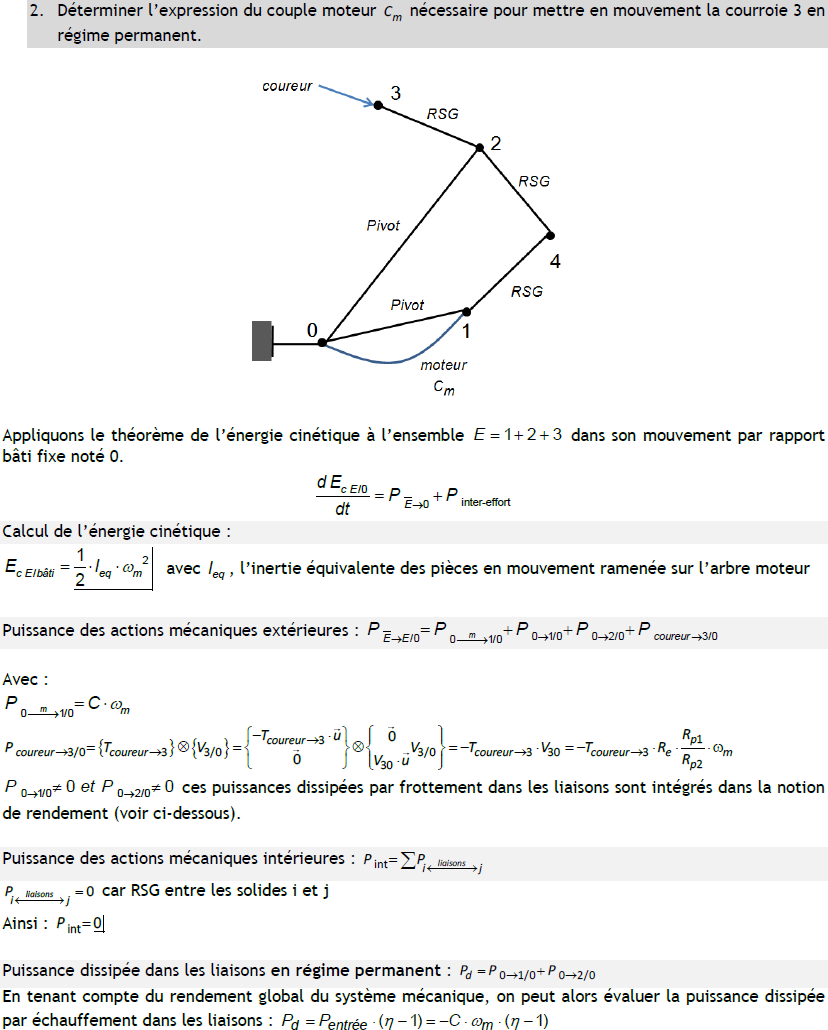
\includegraphics[width=.45\linewidth]{cor_02}
%\textit{}
\end{center}

\end{corrige}
\else
\fi

\question{Donner l’expression littérale de la masse équivalente $M_e'$ et faire l’application numérique.}
\ifprof
\begin{corrige}~\\
En prenant un contrepoids de même masse que l'ascenseur et en négligeant l'inertie de la poulie, le contrepoids se déplaçant à la même vitesse que l'ascenseur (mais dans un sens opposé), on a
$M_e' = \left( J_R+J_V\right) \dfrac{4\pi^2}{p_v^2} +2M$, soit $M_e' = \SI{677}{kg}$
\end{corrige}
\else
\fi

\question{En supposant que toutes les liaisons sont parfaites, déterminer l’expression littérale de $C$ en fonction de $V$ et/ou de ses dérivées, $\omega$ et/ou ses dérivées n’apparaîtront pas dans l’expression littérale de $C$.}
\ifprof
\begin{corrige}~\\
Par rapport au TEC effectué précédemment, il faut ajouter la puissance des actions de pesanteurs sur le contrepoids.
Cette puissance est opposée à la puissance des actions de pesanteur sur l'ascenseur.
 $C = \dfrac{p_v}{2\pi}M_e' \dot{V}$.
 
\end{corrige}
\else
\fi

\question{En déduire la valeur du couple maximum $C_{\text{Max}}$ que le moteur doit pouvoir
appliquer sur la vis ainsi que la puissance $P_0$ nécessaire de ce moteur.}
\ifprof
\begin{corrige}~\\
$C_{\text{Max}} = \SI{0,24}{Nm}$, $P_0 = \SI{38}{W}$.

\end{corrige}
\else
\fi

\question{En déduire la puissance nécessaire $P$ du moteur si le rendement du dispositif vis-écrou vaut $\eta=0,3$.}
\ifprof
\begin{corrige}~\\
Avec les mêmes précautions que précédemment, $P=\SI{127}{W}$. 
\end{corrige}
\else
\fi



\question{Le contrepoids sera réalisé dans un alliage de masse volumique $\SI{9e3}{kg.m^3}$. L’emplacement disponible est un parallélépipède rectangle de
section $0,2 \times \SI{0,1}{m^2}$ et de hauteur \SI{1,4}{m}. Cette solution est-elle envisageable ?}
\ifprof
\begin{corrige}~\\
Au vu de la section disponible, la hauteur du contrepoids sera de $\dfrac{130}{0,1\times 0,2 \times \num{9e3}}=\SI{0,72}{m}$. Le contrepoids doit pouvoir se déplacer de $\SI{0,8}{m}$ soit un encombrement total de \SI{1,52}{m}  supérieur à \SI{1,4}{m} disponible.
\end{corrige}
\else
\fi

\subsection*{Motorisation assistée par un ressort de traction}
Dans cette solution un ressort, travaillant en traction, est choisi pour compenser
le poids de l’ascenseur. Une courroie crantée s’enroule sur un demi-tour
d’une poulie d’axe fixe par rapport au bâti. Une des extrémités de cette courroie
est attachée à l’ascenseur, l’autre à l’une des extrémités du ressort.

\question{Faire un schéma de principe du dispositif.}
\ifprof
\begin{corrige}~\\
~\\
\begin{center}
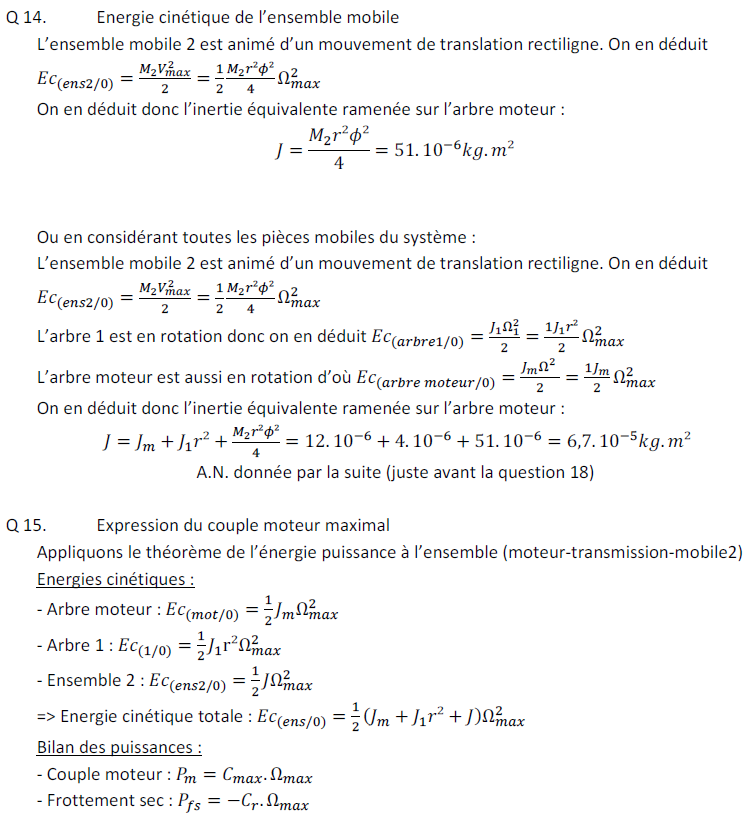
\includegraphics[width=.45\linewidth]{cor_03}
%\textit{}
\end{center}

\end{corrige}
\else
\fi



\question{L’effort minimal développé par le ressort doit compenser exactement le poids
de l’ascenseur. La variation de l’effort de compensation, exercé par le ressort,
sera limitée à 10\,\% sur l’ensemble de la course. Déterminer la raideur du ressort,
ainsi que l’effort de compensation maximum $F_{\text{c maxi}}$ qu’il exercera. Représenter
la courbe de variation de cet effort en fonction du déplacement $y$ de l’ascenseur.}
\ifprof
\begin{corrige}~\\
La course maximale est de \SI{0,8}{m}. La charge à compenser correspond au poids de l'ascenseur soit $Mg$. 
Lorsque l'ascenseur sera en bas, $y$ sera minimal et le ressort sera tendu. L'effort sera donc maximal, soit $1,1 Mg$.
Lorsque l'ascenseur sera en haut, $y$ sera maximal et le ressort sera  << au repos >>. L'effort doit compenser le poids.
La raideur doit être de la forme $k=\dfrac{1,1Mg - Mg}{0,8} = \dfrac{0,1 \times 130 \times 9,81 }{0,8}\simeq \SI{159,4}{N.m^{-1}}$.
\begin{center}
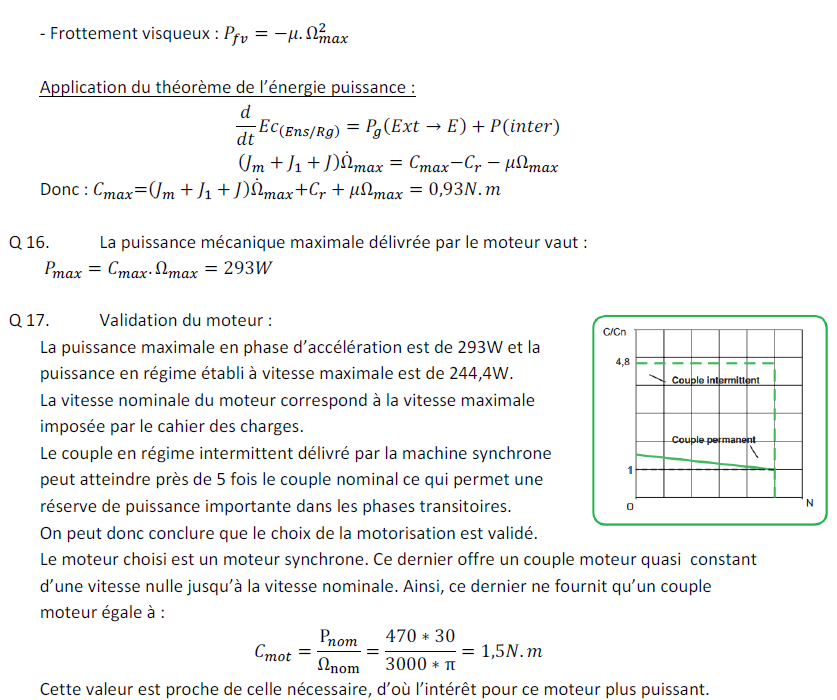
\includegraphics[width=5cm]{cor_04}
%\textit{}
\end{center}
\end{corrige}
\else
\fi

\ifprof
\else
L’emplacement disponible ne permet pas de placer un ressort de diamètre
nominal $D$ supérieur à \SI{0,1}{m}. Le ressort de traction sera réalisé dans un acier
allié de résistance élastique au glissement $R_{eg}=\SI{560}{MPa}$ et de module de Coulomb $G=\SI{82000}{MPa}$. On prendra un coefficient de sécurité $s=2$. Pour que le
ressort résiste à l’effort maximal $F_{\text{c maxi}}$, il doit avoir un diamètre
$d\geq \sqrt[3]{\dfrac{8 F_{\text{c maxi}} D s}{\pi R_{eg}}}$, 
c'est-à-dire $d\geq 9,7 \times 10^{-4}\sqrt[3]{F_{\text{c maxi}}}$.

Pour obtenir un ressort de raideur $r$ il faut un nombre de spires $n=\dfrac{Gd^4}{8D^3 r}$, c'est-à-dire $n\simeq 10^{13}\dfrac{d^4}{r}$.

\fi
\question{La longueur du ressort est-elle compatible avec l’emplacement disponible ?}
\ifprof
\begin{corrige}~\\
Dans les conditions proposées ci-dessus, on a $d=9,7 \times 10^{-4}\sqrt[3]{1,1\times Mg}= \SI{0,011}{m}$. 
Le nombre de spires serait alors $n=872$. Si les spires sont jointives, on a une longueur de ressort minimale de $dn =\SI{9,47}{m}$ ce qui dépasse très largement les dimensions de la machine.  
\end{corrige}
\else
\fi

\subsection*{Assistance à l’aide d’un vérin à gaz}
\ifprof
\else
Le schéma de principe de ce dispositif a été donné précédemment. Le corps du vérin est lié au bâti. Une poulie crantée
est en liaison pivot avec l’extrémité de la tige du vérin. Une courroie crantée s’enroule (un demi-tour) sur la poulie et est liée au bâti à une de ses extrémités. L’autre extrémité de la courroie est liée à l’ascenseur.
\fi

\question{Déterminer la relation existant entre le déplacement $y$ de l’ascenseur et le
déplacement $y_T$ de la tige du vérin. En déduire la course $\Delta y_T$ nécessaire de la tige du vérin à gaz.}
\ifprof
\begin{corrige}~\\

En utilisant le roulement sans glissement de la poulie par rapport à la courroie en $I$ on montre que $y_T = \dfrac{1}{2}y$.
\begin{center}
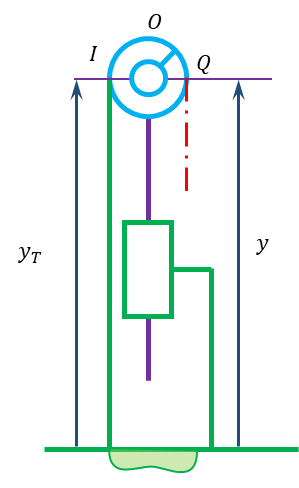
\includegraphics[width=3cm]{cor_05}
%\textit{}
\end{center}
\end{corrige}
\else
\fi


\question{Le module de l’effort appliqué par la courroie sur l’ascenseur est noté $F_c$.
C’est l’effort de compensation sur l’ascenseur. En isolant la poulie, déterminer
la relation existant entre l’effort $F$ développé par le vérin et l’effort de compensation $F_c$. 
%Compléter alors, le bloc 12b du schéma-bloc du document réponse. 
En déduire l’effort minimum $F_{\text{mini}}$ développé par le vérin.}

\ifprof
\begin{corrige}~\\

\begin{center}
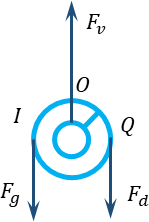
\includegraphics[width=3cm]{cor_06}
%\textit{}
\end{center}

Si on néglige la masse de la poulie, on peut appliquer le PFS (à la place du PFD).

\begin{itemize}
\item On isole la poulie de rayon $R$.
\item La poulie est soumise au brin de gauche, au brin de droite et à l'effort du vérin.
\item TMS en O, centre de la pivot : $F_g R -R F_d = 0$ soit $F_g =F_d$. 
\item TRS : $2F_d+ F_v = 0$. 
\end{itemize}
En reprenant les notations de la question, on a $2F_c = F$.
Comme au minimum, $F_c = Mg$, on a donc $F_{\text{mini}} = 2 Mg = \SI{2550,6}{N}$.
\end{corrige}
\else
\fi

\ifprof
\else
Le vérin à gaz est présenté sur le dessin ci-dessous.
\begin{center}
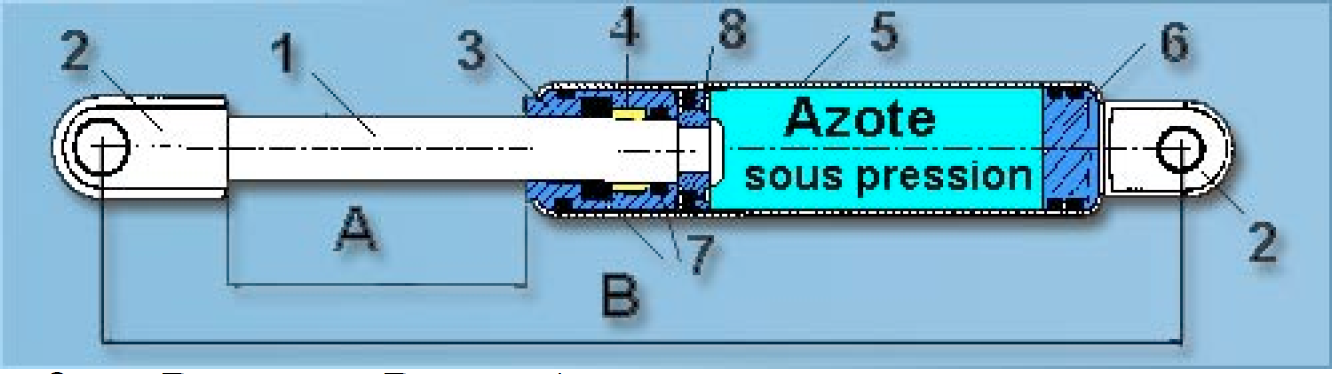
\includegraphics[width=\linewidth]{fig_11}
\end{center}
\fi

\question{Pour étudier l’action exercée par l’azote sous pression sur la tige du vérin on
propose les deux modèles ci-dessous. Montrer que lorsque la tige n’est pas
en mouvement ces deux modèles de comportement du vérin à gaz, sont équivalents
du point de vue des actions qu’exerce l’azote sur la tige du vérin.
Remarque : pour la suite de cette étude on négligera les pertes de charge lors de
l’écoulement du fluide à travers l’orifice du piston.}
\ifprof
\begin{corrige}~\\
Soit $D$ le diamètre du vérin et $d$ le diamètre de la tige. 

Dans le premier cas, on a, dans la chambre droite, $F_d = + p \pi\dfrac{D^2 - d^2}{4}$ et $F_g =- p \pi\dfrac{D^2}{4}$. La résultante des forces est donc  $F_g +F_d=-p \pi\dfrac{d^2}{4}$.

Dans le second cas, l'effort est $-p \pi\dfrac{d^2}{4}$. Les deux modèle sont donc équivalent.
\end{corrige}
\else
\fi

\ifprof
\else
\begin{center}
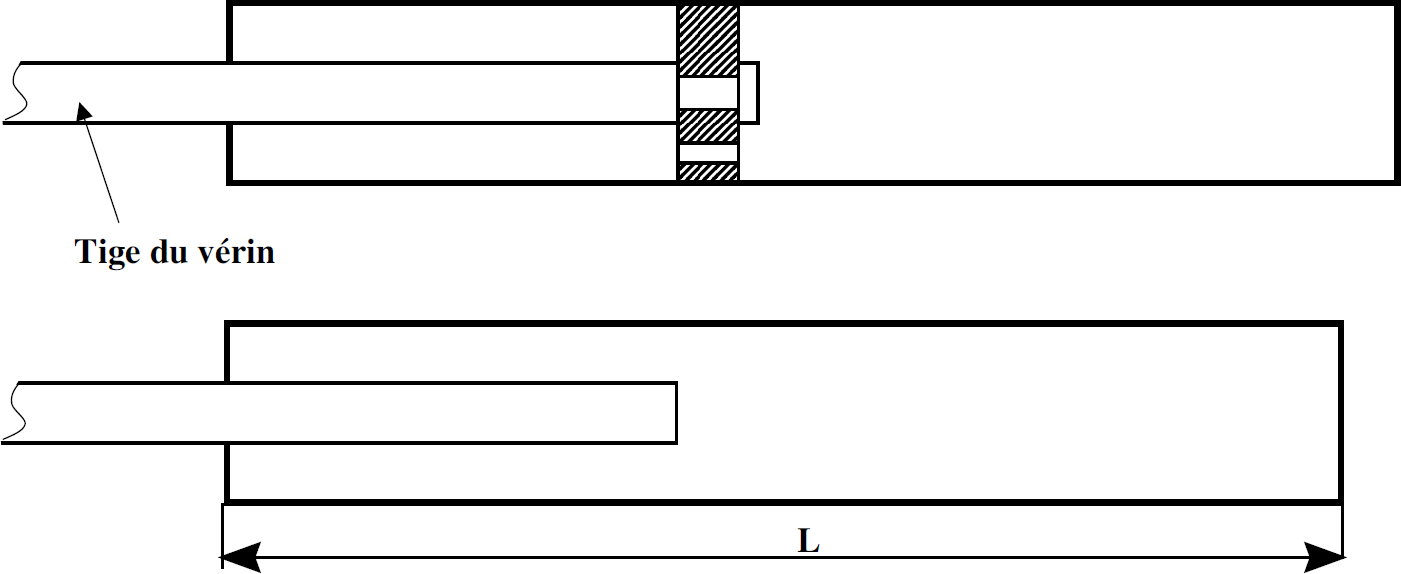
\includegraphics[width=\linewidth]{fig_12}
\end{center}
\fi

\question{Compte tenu des efforts on pré-dimensionne la tige du vérin à un diamètre $d=\SI{15e-3}{m}$. On appelle pression de gonflage, la pression de l’azote que le
vérin contient quand la tige est complètement sortie. Déterminer la pression de
gonflage du vérin, cette pression sera notée $p_2$.}
\ifprof
\begin{corrige}~\\
On a $p_2 = \dfrac{F_{\text{mini}}}{\dfrac{\pi d^2}{4}}$ $=\SI{14433443}{Pa}$ soient \SI{144}{bars}.
\end{corrige}
\else
\fi

\ifprof
\else
Dans la gamme de vérin à gaz on choisit le vérin de diamètre le plus grand
$D=\SI{57e-3}{m}$. L’espace disponible permet de placer un vérin dont la chambre
a une longueur maximale $L=\SI{1}{m}$. Soient $p_1$, $F_1$, $V_1$ la pression,
l’effort de poussée du vérin et le volume de gaz dans le vérin pour la position
ascenseur en bas et $p_2$, $F_{\text{mini}}$, $V_2$ pour la position ascenseur en haut. Pour cette
position, la tige du vérin est complètement sortie.
\fi


\question{Donner l’expression littérale
de la raideur de ce vérin à gaz en fonction de $F_1$, $F_{\text{mini}}$ et $\Delta_{y_T}$. Exprimer $F_{\text{mini}}$
en fonction de $p_2$ et d’une caractéristique géométrique du vérin. Exprimer $F_1$
en fonction de $p_1$ et d’une caractéristique géométrique du vérin. On suppose que
la transformation de l’azote entre les états 1 et 2 est isotherme. Donner
l’expression littérale de la raideur $r$ de ce vérin à gaz en fonction de $F_{\text{mini}}$, $d$,
$D$, $L$ et $\Delta_{y_T}$.}
\ifprof
\begin{corrige}~\\
\begin{itemize}
\item $r=\dfrac{F_1-F_{\text{mini}}}{\Delta y_T}$.
\item $F_{\text{mini}}=p_2\dfrac{\pi d^2}{4}$, $F_1=p_1\dfrac{\pi d^2}{4}$.
\item On a $p_1 V_1 = p_2 V_2$  $\Leftrightarrow F_{\text{mini}} V_1 = F_1 V_2$ $\Leftrightarrow F_{\text{mini}} \dfrac{V_1}{V_2} = F_1$. D'où $r=\dfrac{F_{\text{mini}} \dfrac{V_1}{V_2}-F_{\text{mini}}}{\Delta y_T}$
$F_{\text{mini}}\dfrac{ \dfrac{V_1}{V_2}-1}{\Delta y_T}$.
\end{itemize}
Par ailleurs, $V_1-V_2=\Delta y_T \dfrac{\pi d^2}{4}$; donc $V_2 = L\dfrac{\pi D^2}{4}-\Delta y_T \dfrac{\pi d^2}{4}$.

On a donc $r=F_{\text{mini}}\dfrac{ \dfrac{V_1-V_2}{V_2}}{\Delta y_T}$ $ =F_{\text{mini}}\dfrac{ \dfrac{\Delta y_T \dfrac{\pi d^2}{4}}{ L\dfrac{\pi D^2}{4}-\Delta y_T \dfrac{\pi d^2}{4}}}{\Delta y_T}$ 
$ =F_{\text{mini}}\dfrac{ \dfrac{\Delta y_T  d^2}{ L D^2-\Delta y_T d^2}}{\Delta y_T}$ 
$ =F_{\text{mini}}\dfrac{ d^2}{ L D^2-\Delta y_T d^2}$ 
\end{corrige}
\else
\fi

\question{On cherche à obtenir une raideur la plus faible possible, choisir alors la longueur $L$
et calculer la raideur $r$.}
\ifprof
\begin{corrige}~\\
Pour avoir la raideur la plus faible, il faut la longueur la plus grande soit $\SI{1}{m}$.
$r =F_{\text{mini}}\dfrac{ d^2}{ L D^2-\Delta y_T d^2}$ 
\end{corrige}
\else
\fi

On prendra $r=\SI{180}{Nm^{-1}}$ pour la suite du problème.

\question{Déterminer l’effort maximal $F_{\text{Maxi}}$ développé par le vérin. Faire l’application
numérique. Calculer la variation en \% de $F$.}
\ifprof
\begin{corrige}~\\
$F_{\text{Maxi}}  =F_{\text{Mini}}+r\Delta y_T$ $=2550+180\time 0,4 = \SI{2622}{N}$.

La variation d'effort est de $\dfrac{72}{2550}\simeq 3\,\%$. 
\end{corrige}
\else
\fi

\question{Déterminer la relation $F=F(y_T)$.}
% Compléter alors, l’entrée et le bloc du schéma-bloc du document réponse.}
\ifprof
\begin{corrige}~\\
$F=2622-r y_T$.
\end{corrige}
\else
\fi

On considérera dans cette question que l’effort de compensation $F_c$ est constant.

\question{En supposant que toutes les liaisons sont parfaites, déterminer l’expression
littérale de $C$ en fonction de $a$, $M_e$, $F_c$, $M$...}
\ifprof
\begin{corrige}~\\
En reprenant l'expression précédente et en ajoutant l'effort de la courroie $F_c$ (de sens opposé au poids), on a 
$C = \dfrac{p_v}{2\pi}\left(M_e \dot{V} +Mg-F_c\right) $.
\end{corrige}
\else
\fi

\question{Exprimer ensuite $a$ en fonction de $C$, $M_e$, $F_c$, $M$ ...}
\ifprof
\begin{corrige}~\\
On a $a=\dot{V}$ et $a=\dfrac{1}{M_e}\left( \dfrac{2\pi C}{p_v}+F_c-Mg \right)$.
\end{corrige}
\else
\fi

\question{En déduire la valeur du couple maximum $C_{\text{Max}}$ que le moteur doit pouvoir
appliquer sur la vis ainsi que la puissance $P_0$ nécessaire de ce moteur (prendre $F_c = \SI{1300}{N}$).}
\ifprof
\begin{corrige}~\\
On reprend l'expression de $C$ et on a $C=\SI{0,22}{Nm}$.
$P_0=\SI{34,4}{W}$
\end{corrige}
\else
\fi

\question{En déduire la puissance $P$ nécessaire du moteur si le rendement du dispositif
vis-écrou vaut $\eta=0,3$.}
\ifprof
\begin{corrige}~\\
$P=\SI{115}{W}$
\end{corrige}
\else
\fi
\subsection*{Synthèse}

\question{On se propose de résumer l’étude comparative précédente dans un tableau. Indiquer les valeurs calculées pour la puissance du moteur, le couple du moteur, la masse équivalente. On rappelle que
le calcul de la masse équivalente a été effectué en prenant l’inertie de la vis
dimensionnée pour la solution avec vérin à gaz. Compte tenu de cette remarque,
indiquer si la masse équivalente, trouvée en réponse aux questions précédentes,
a été obtenue par excès ou par défaut. L’encombrement est-il (oui ou non) compatible
avec le cahier des charges ? La masse de l’ensemble est-elle
satisfaisante ?}
\ifprof
\begin{corrige}~\\
\end{corrige}
\else
\fi

%\question{}
%\ifprof
%\begin{corrige}~\\
%\end{corrige}
%\else
%\fi
%
%
%
%%
%\question{}
%\ifprof
%\begin{corrige}~\\
%\end{corrige}
%\else
%\fi

\ifprof
\else
\end{multicols}
\fi